\chapter{Introducción}
\label{chap:introduccion}

\drop{C}{}ada vez es más habitual que se produzcan \textbf{cataclismos atmosféricos} \cite{desastres} que puedan provocar la pérdida de vidas, como incendios, terremotos, inundaciones o tsunamis. Además, a estas catástrofes naturales se le añaden los \textbf{factores de riesgo provocados por los humanos} durante el ejercicio de actividades industriales \cite{desastres}, como puede ser un accidente nuclear.
  
Los momentos inmediatamente posteriores a la ocurrencia de estas catástrofes son extremadamente críticos para minimizar el daño causado. Normalmente, existe un protocolo de actuación, bien definido, basado en la coordinación de personal especializado y la gestión de recursos, para responder de manera eficiente cuando tiene lugar una catástrofe. Por ejemplo, en el caso de un terremoto resulta esencial la intervención inmediata de un equipo de rescate para maximizar el número de personas rescatadas con vida. No obstante, \textbf{la actuación humana resulta muy complicada en determinadas circunstancias} debido a las propias consecuencias de la catástrofe y al riesgo real para el personal responsable de gestionar la crisis.

Este tipo de entornos son ideales para \textbf{emplear vehículos aéreos no tripulados (\acs{UAV}s)}, más comúnmente llamados drones, ya que en este contexto la tecnología puede contribuir a mejorar dicha gestión gracias al soporte de drones autónomos, que sirvan como primera línea de actuación para recabar información, en escenarios poco accesibles, de una forma rápida y lo más precisa posible. Si además esta intervención se realiza de manera coordinada, las probabilidades de minimizar los daños de la catástrofe sufrida crecen considerablemente.

Los drones, generalmente, exhiben una \textbf{capacidad de respuesta en tiempo record} y continuamente están aportando nuevas oportunidades para el apoyo, que mediante el uso de otros recursos sería inviable o poco efectivo. En cuanto al empleo de cámaras, los drones son capaces de trabajar con termografía, visión nocturna, multiespectrales, réflex, etc.

En la actualidad, existen sistemas de drones capaces de transportar salvavidas desde la playa hasta varios kilómetros mar adentro \cite{dronsocorrista}, y que confirman que es plausible una \textbf{asistencia más rápida} que una moto de agua.\\

El ayuntamiento de Madrid se ha convertido en el primer consistorio en proporcionar un \acs{UAV} cuyo uso se extiende al Cuerpo de Bomberos, Samur y Policía Municipal. Se enmarca en el proyecto piloto SOS Drone \cite{sosdrone} y es capaz de \textbf{actuar en condiciones adversas} como altas temperaturas, humos, contaminantes y tóxicos. El dron fue utilizado por primera vez en septiembre de 2013 en la Puerta de Alcalá durante la elección de la sede de los Juegos Olímpicos de 2020.

En este \acs{TFG} se propone la creación de un \textbf{sistema que permita un despliegue coordinado} de varios \acs{UAV}s para conseguir información útil sobre el entorno damnificado por el desastre. A través del equipamiento de cámaras, en drones, se pueden llevar a cabo misiones de búsqueda y rescate, maximizando las posibilidades de éxito de la misión iniciada y reduciendo ostensiblemente el coste operacional.

\section{Contexto}
\label{sec:contexto}

El contexto del \acs{TFG} está enfocado a la \textbf{utilización y coordinación de \acs{UAV}s en situaciones de emergencias}, por ejemplo desastres naturales o provocados por el ser humano. Los científicos han confirmado que estos sucesos han \textbf{aumentado de manera preocupante} en las últimas décadas \cite{aumento}.

Para constatar este hecho, en la Figura~\ref{fig:catastrofesnat} se observa la evolución en la cantidad de desastres naturales identificados desde el año 1900 hasta el año 2015. En esta gráfica se advierte un incremento mayúsculo de este tipo de catástrofes en los últimos 30 años.

\begin{figure}[!h]
\begin{center}
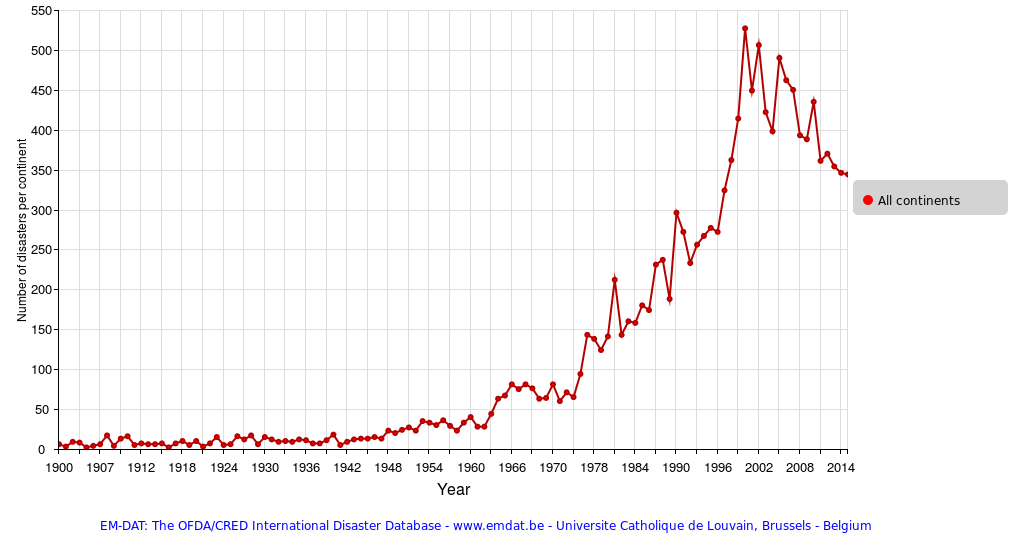
\includegraphics[width=0.8\textwidth]{/catastrofesnaturales.png}
\caption[Número de desastres naturales registrados en el periodo 1900-2015]{Número de desastres naturales registrados en el periodo 1900-2015 \footnotemark}
\label{fig:catastrofesnat}
\end{center}
\end{figure}

\footnotetext{\url{http://www.emdat.be/disaster\_trends/index.html}}

\clearpage

Con el auge existente en torno a los drones, en la sociedad actual, \textbf{se abre todo un mundo de posibilidades para la creación de sistemas} que sean útiles para la humanidad. Según Sophic Capital (ver Figura~\ref{fig:previsioningresos}), los ingresos totales de las compañías que trabajan con \acs{UAV}s pueden ascender hasta más de 12.000 millones de dólares en el año 2025.
 
\begin{figure}[!h]
\begin{center}
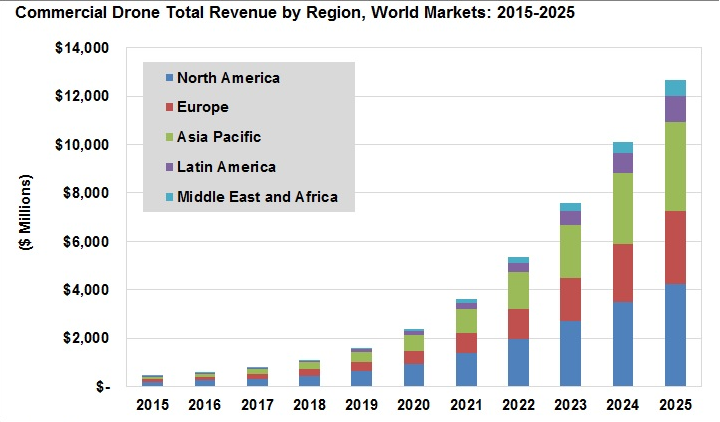
\includegraphics[width=0.8\textwidth]{/DCA-15-chart.png}
\caption[Previsión de ingresos por regiones en el periodo 2015-2025]{Previsión de ingresos por regiones en el periodo 2015-2025 \cite{cuotamercado}}
\label{fig:previsioningresos}
\end{center}
\end{figure}

Aprovechando sus ventajas, los drones constituyen una \textbf{valiosa ayuda para los cuerpos de seguridad} del Estado, los ciudadanos, y en conclusión implican un gran avance para todos, algo que se demuestra hoy en día, dado que, evitan muchas pérdidas humanas.

\section{Motivación}
\label{sec:motivacion}

Estimar el tiempo de actuación en labores de socorro es una tarea compleja, pero los drones pueden \textbf{desplegarse con rapidez} y acortar sustancialmente el tiempo de respuesta y el riesgo de lesiones de los individuos desaparecidos y de los equipos de rescate. En el caso de rescates acuáticos, según la empresa Vodafone, responsable de un proyecto piloto que utiliza drones para ayudar a rescatar a los bañistas en apuros, «un socorrista tarda el triple de tiempo que un dron necesita para llegar a un bañista en peligro» \cite{tiempomenor}.

Los \acs{UAV}s son un \textbf{aliado perfecto en misiones de búsqueda y rescate} puesto que sus limitaciones en condiciones meteorológicas adversas son menores. Aparte de esto, el uso de sensores especializados contribuyen a equipar los \acs{UAV} de ventajas importantes en la realización de este tipo de operaciones. Sirva como precedente «la utilización de helicópteros no tripulados franceses Elipse HE 300 durante la actual crisis de la central de Fukushima» \cite{notripulados}.

Este tipo de dispositivos, utilizados de manera simultánea con la intervención humana de los equipos de rescate, resultan herramientas vitales a la hora de detectar, localizar y rescatar a víctimas de catástrofes naturales como los terremotos o incidentes como el hundimiento de minas. El auxilio de personas en esta clase de condiciones puede resultar peligroso para los miembros del servicio de respuesta rápida ante emergencias. Sin embargo, los dispositivos no tripulados pueden impedir males mayores y colaborar de manera eficaz con los humanos en condiciones complicadas.

Con todo lo anterior, en este TFG se pretende \textbf{mejorar la productividad de los equipos de rescate}, en situaciones de catástrofe, permitiendo rebajar los tiempos de reconocimiento del terreno con la ayuda de una flota de \acs{UAV}s que se coordinen y comuniquen de forma descentralizada.

El objetivo principal del proyecto es la \textbf{creación de un sistema que permita monitorizar determinadas zonas}, basándose en prioridades, de tal forma que en caso de catástrofe el uso de este software permita reducir costes en cuanto a: i) el tiempo de reconocimiento del territorio afectado por el desastre, ii) el tiempo de rescate de individuos y iii) la exposición al peligro por parte del personal de emergencia.

\section{Estructura del documento}

\begin{definitionlist}
\item[Capítulo \ref{chap:introduccion}: \nameref{chap:introduccion}] Es el presenta capítulo. Se introduce el Trabajo Fin de Grado.
\item[Capítulo \ref{chap:objetivos}: \nameref{chap:objetivos}] Se exponen los objetivos que se aspiran satisfacer una vez concluido el proyecto.
\item[Capítulo \ref{chap:antecedentes}: \nameref{chap:antecedentes}] Se hace un repaso acerca de los antecedentes de la aviación no tripulada, se describe el estado actual de la inteligencia artificial distribuida, se habla sobre los principales sistemas de catástrofes con drones que se han creado y de las herramientas más importantes para el desarrollo de estos sistemas.
\item[Capítulo \ref{chap:metodo}: \nameref{chap:metodo}] Se especifica la metodología, así como los medios hardware y software que han sido utilizados durante el proyecto.
\item[Capítulo \ref{chap:arquitectura}: \nameref{chap:arquitectura}] Se detalla la arquitectura propuesta para el sistema, puntualizando en sus diferentes capas y funciones.
\item[Capítulo \ref{chap:resultados}: \nameref{chap:resultados}] Muestra y explica la evolución del proyecto, los resultados que se han conseguido y el coste total en euros.
\item[Capítulo \ref{chap:conclusiones}: \nameref{chap:conclusiones}] Se enuncian las conclusiones alcanzadas tras haber finalizado el sistema y se proponen posibles actividades a realizar en un futuro.
  %(con todo detalle) del presente documento.
\end{definitionlist}



% Local Variables:
%  coding: utf-8
%  mode: latex
%  mode: flyspell
%  ispell-local-dictionary: "castellano8"
% End:
